\chapter{Pruebas}
En este capitulo se van a mostrar varios casos de uso de la aplicación, junto con las soluciones que obtiene. Dichos casos de uso están basados en los datos de la ciudad de Granada.

\section[Caso 1]{Ruta sobre museos en Granada}
En el caso de que un usuario quiera visitar museos, lo primero que debe hacer es abrir la aplicación y seleccionar un alojamiento; para ello debe levantar o pulsar sobre la pestaña llamada \enquote{Sitios interesantes}. Una vez se ha seleccionado el alojamiento; el usuario deberá buscar en la lista el tipo llamado \enquote{Museos}, al lado de esta hay una casilla en la que deberá pulsar para que se seleccionen todos los museos. El resultado se puede ver en la figura \ref{fig:selec_museos}.\newline

Una vez ha seleccionado los museos deberá pulsar en el botón \enquote{Comenzar búsqueda}. Cuando se haya terminado la búsqueda de la ruta, se cargará otro mapa en el que se mostrará los museos seleccionados en la ruta; si el usuario pulsa en alguno de los marcadores se mostrará el nombre y el horario de entrada y salida del museo aproximada. Si quiere ver la ruta entera en detalle, puede pulsar o deslizar hacia arriba la pestaña \enquote{Descripción ruta final}.\newline

Si nos fijamos en la ruta seleccionada que se muestra en las figuras \ref{fig:salida}; se puede ver que el algoritmo selecciona el primer museo que se encuentra más cerca del alojamiento seleccionado, después va seleccionando el museo más cercano al que se ha visitado; cumpliendo con la heurística que se ha implementado.
\begin{figure}[H]
	\centering
	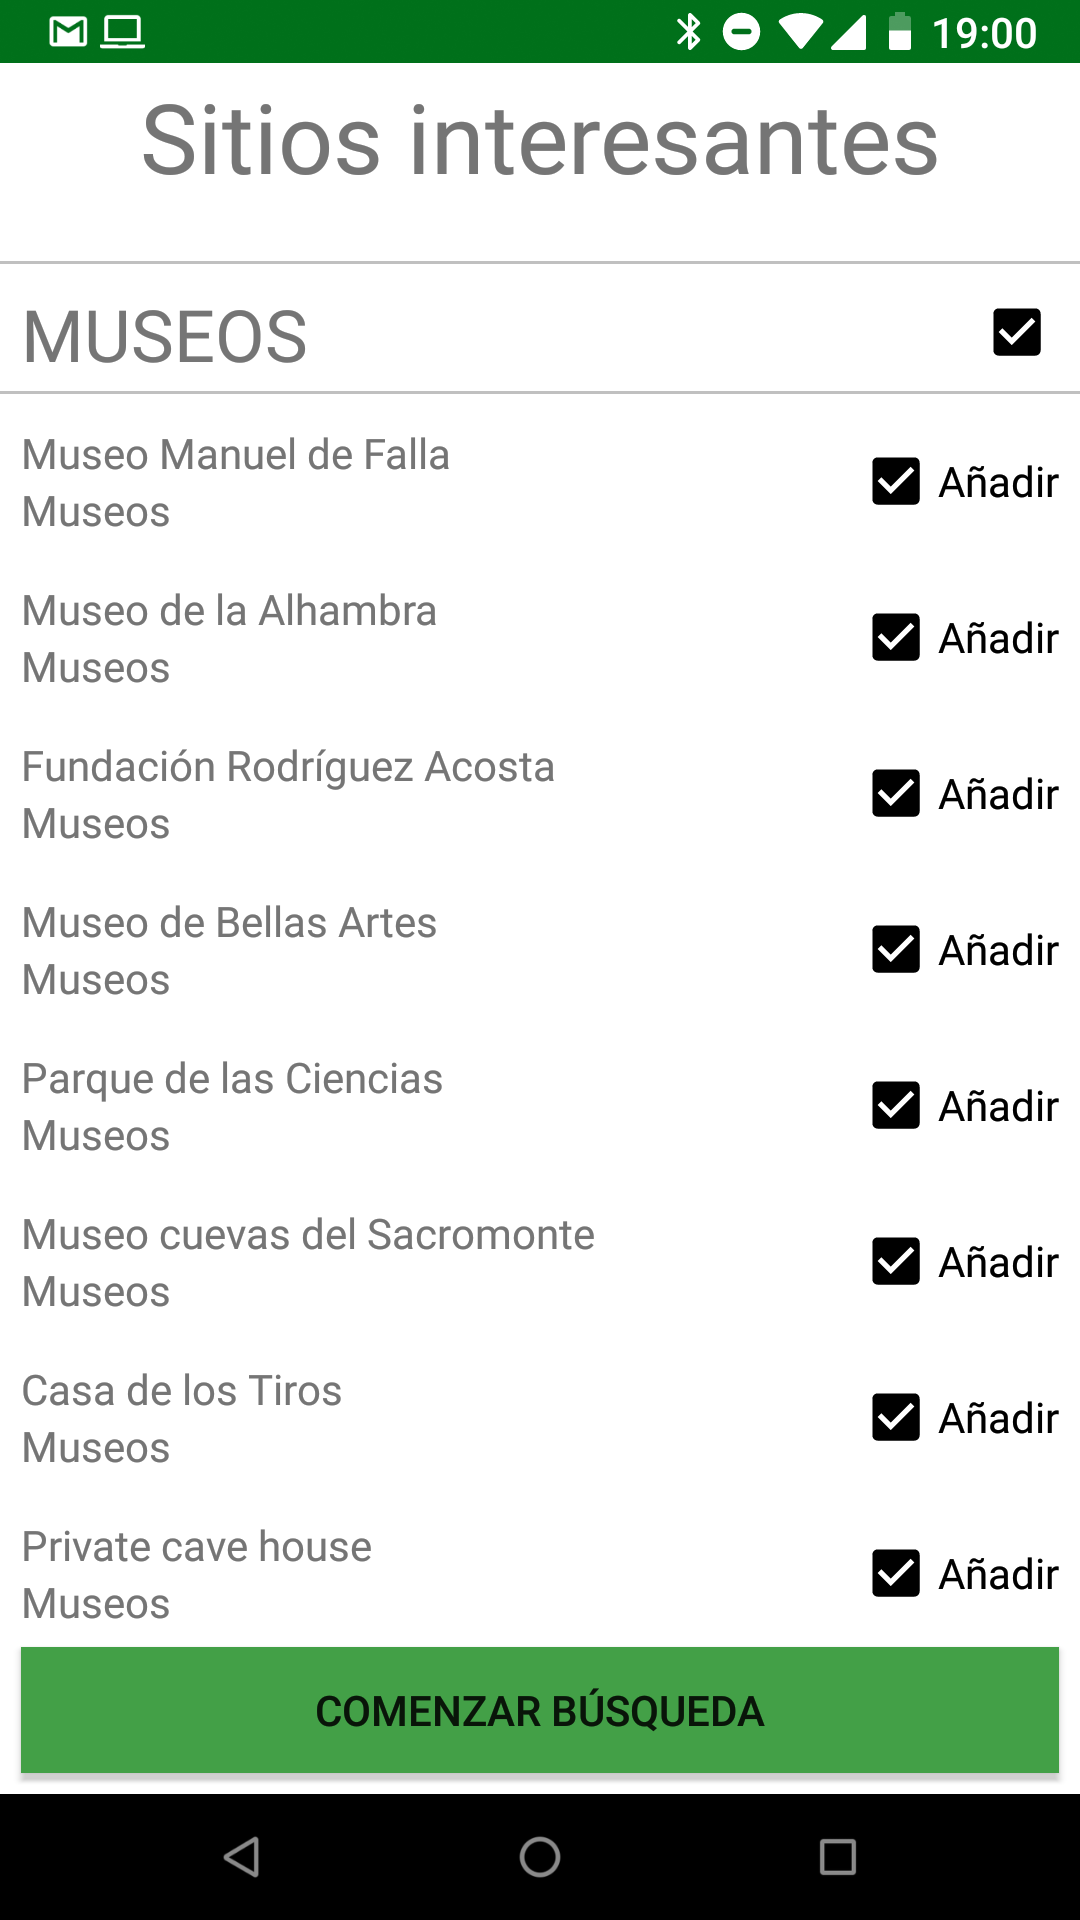
\includegraphics[width=50mm]{imagenes/seleccion_museos}
	\caption{Selección de todos los museos disponibles dentro de la aplicación.}
	\label{fig:selec_museos}
\end{figure}
\begin{figure}[H]
	\centering
	\subfigure{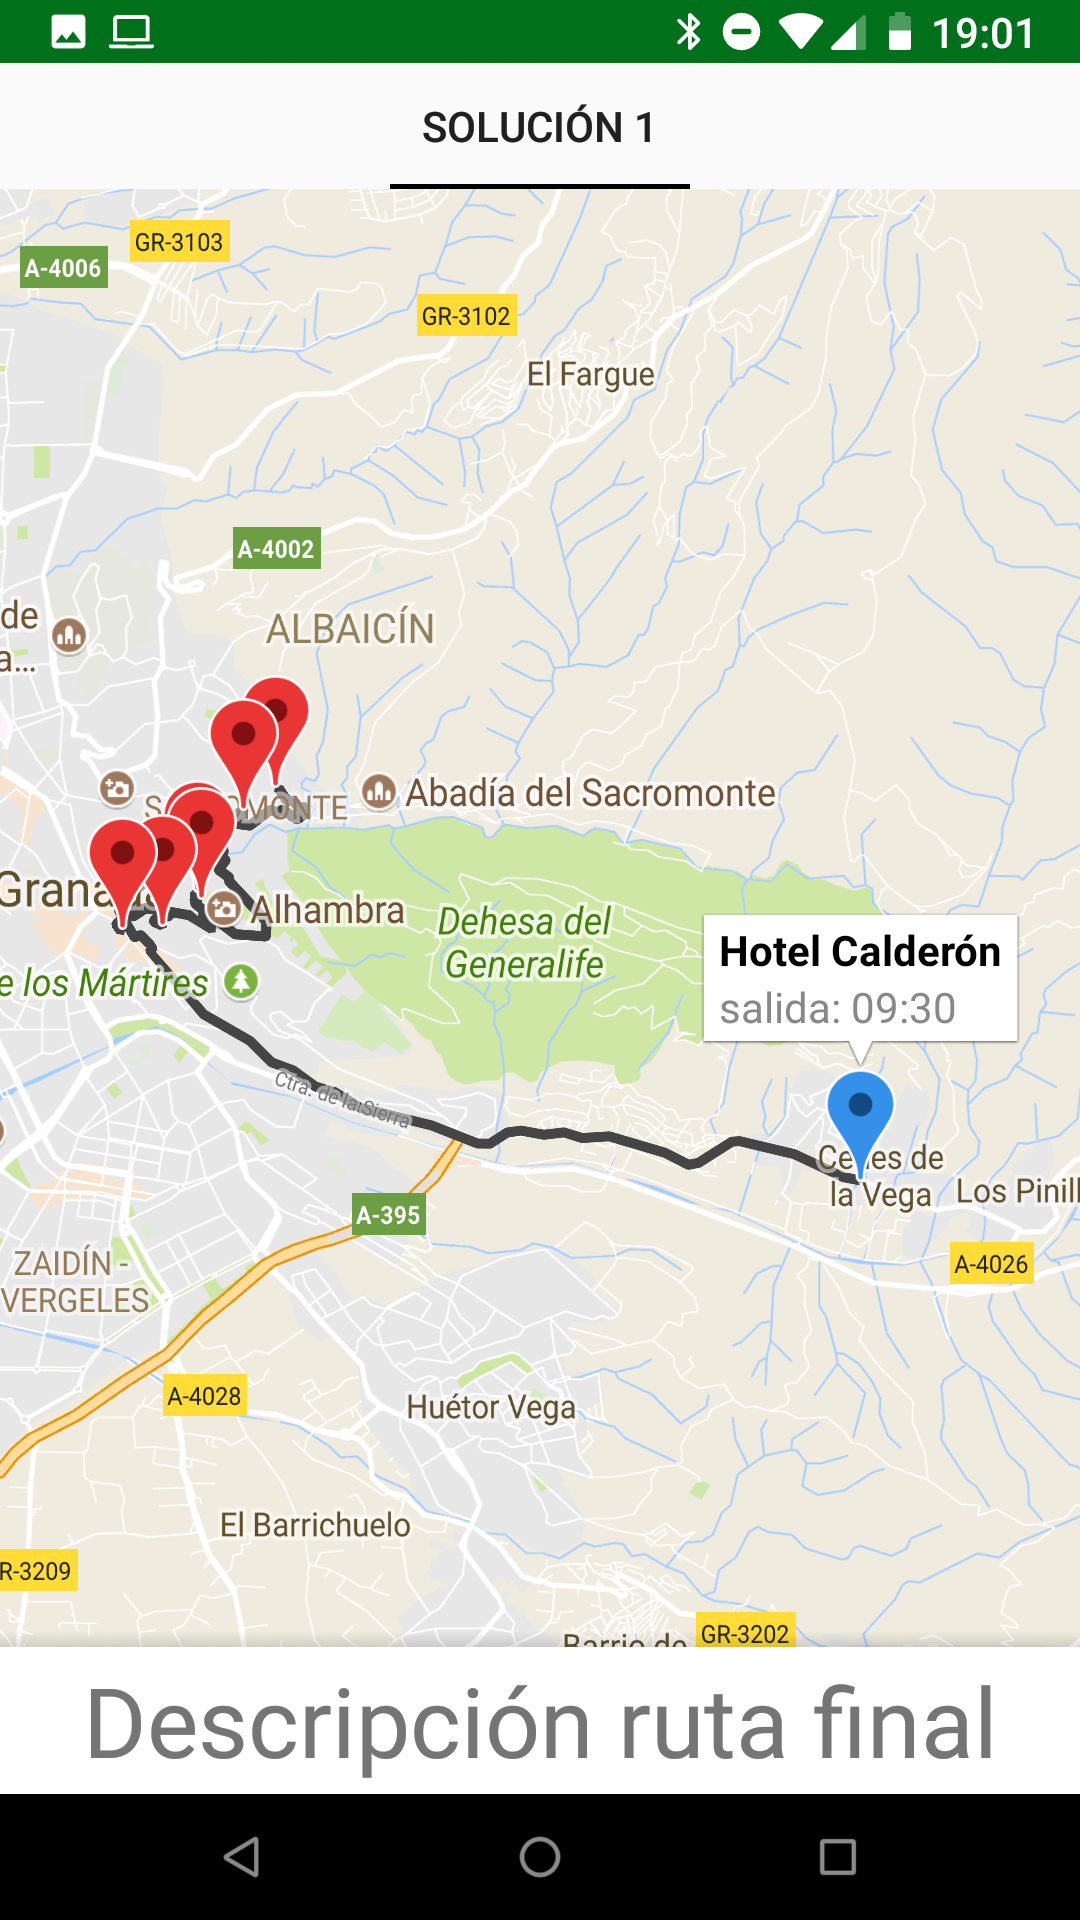
\includegraphics[width=40mm]{imagenes/salida_1}}
	\subfigure{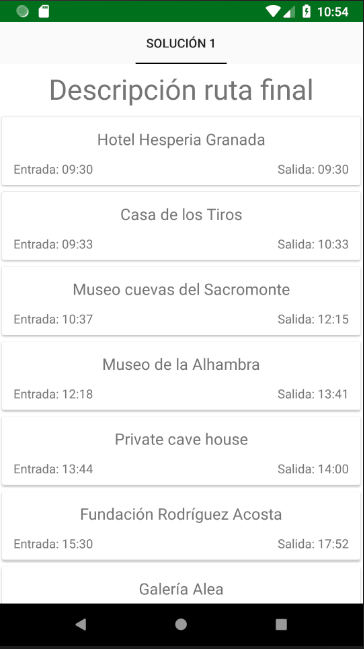
\includegraphics[width=40mm]{imagenes/descripcion_ruta}}
	\caption{Ruta obtenida para el alojamiento seleccionado y todos los museos seleccionados.}
	\label{fig:salida}
\end{figure}

\section[Caso 2]{Ruta sobre un conjunto específico de puntos de interés}
\begin{figure}[H]
	\centering
	\subfigure{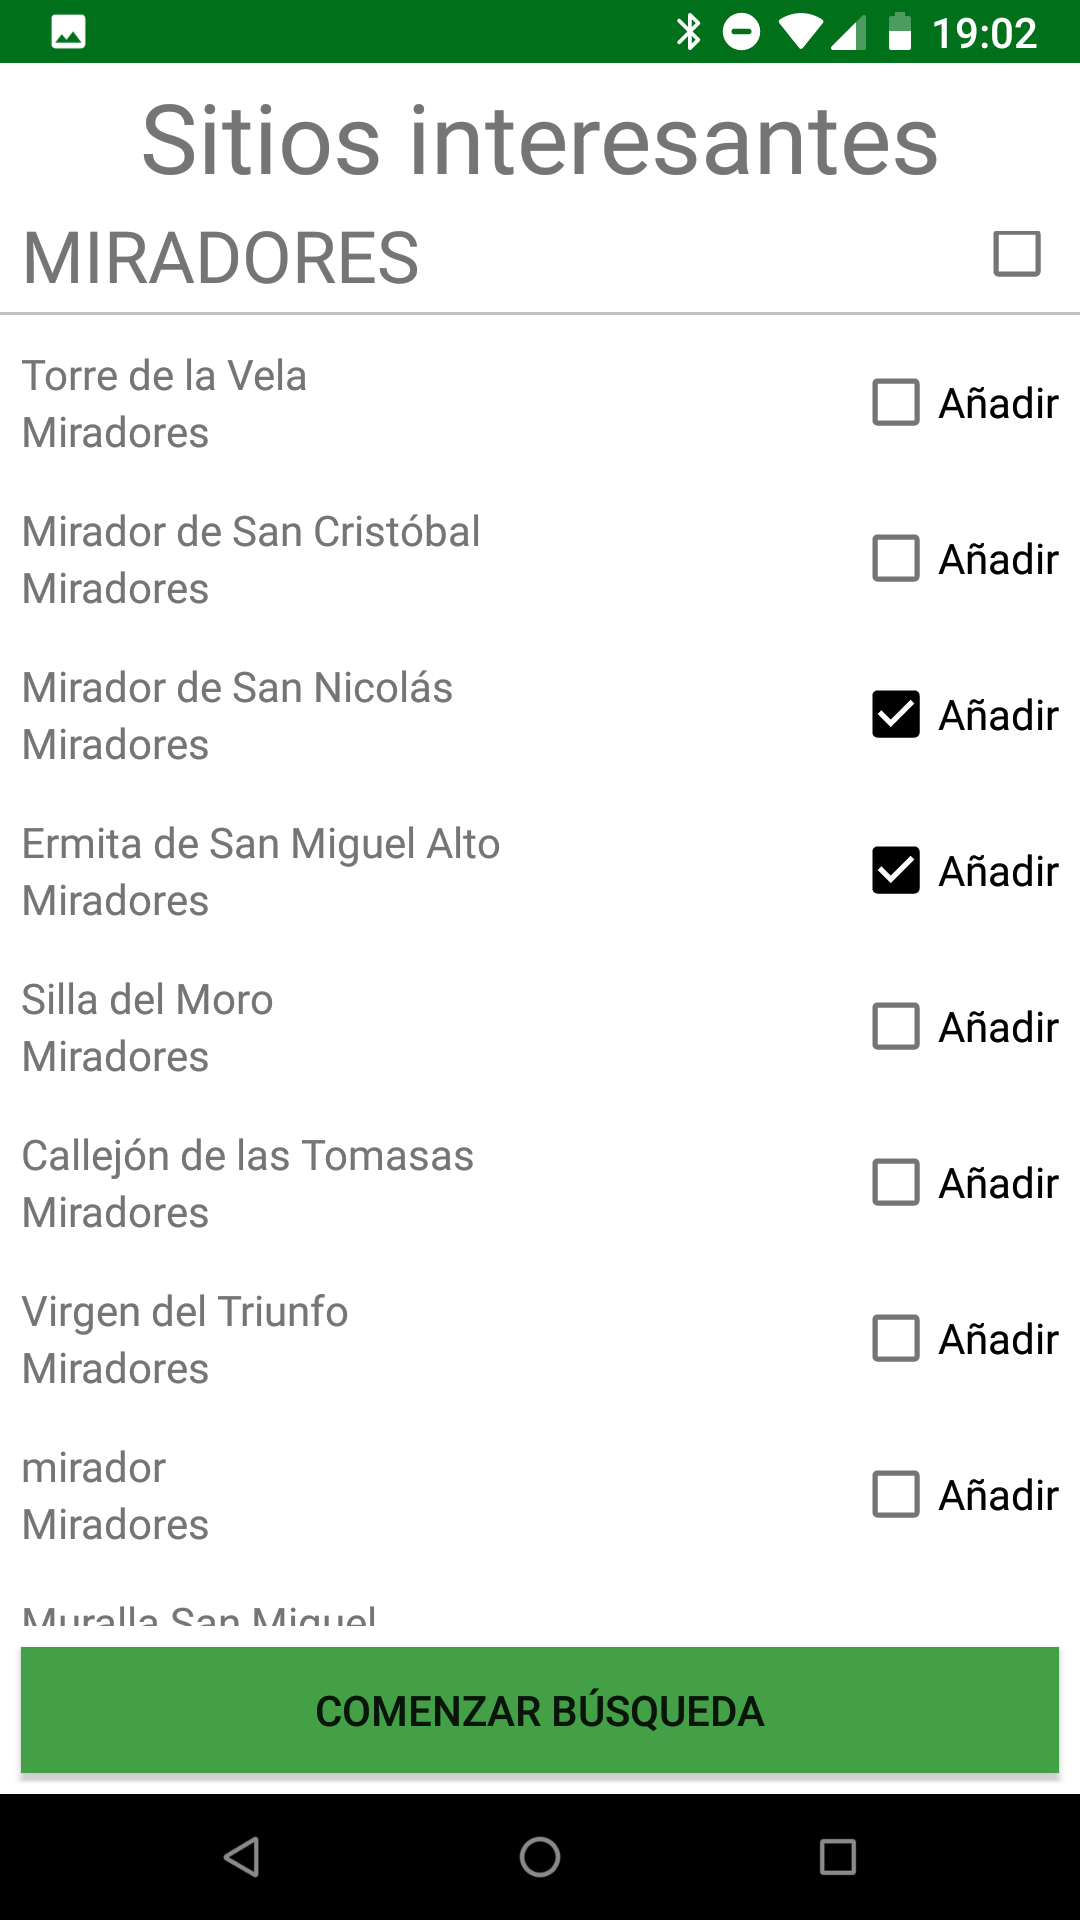
\includegraphics[width=40mm]{imagenes/seleccion_miradores}}
	\subfigure{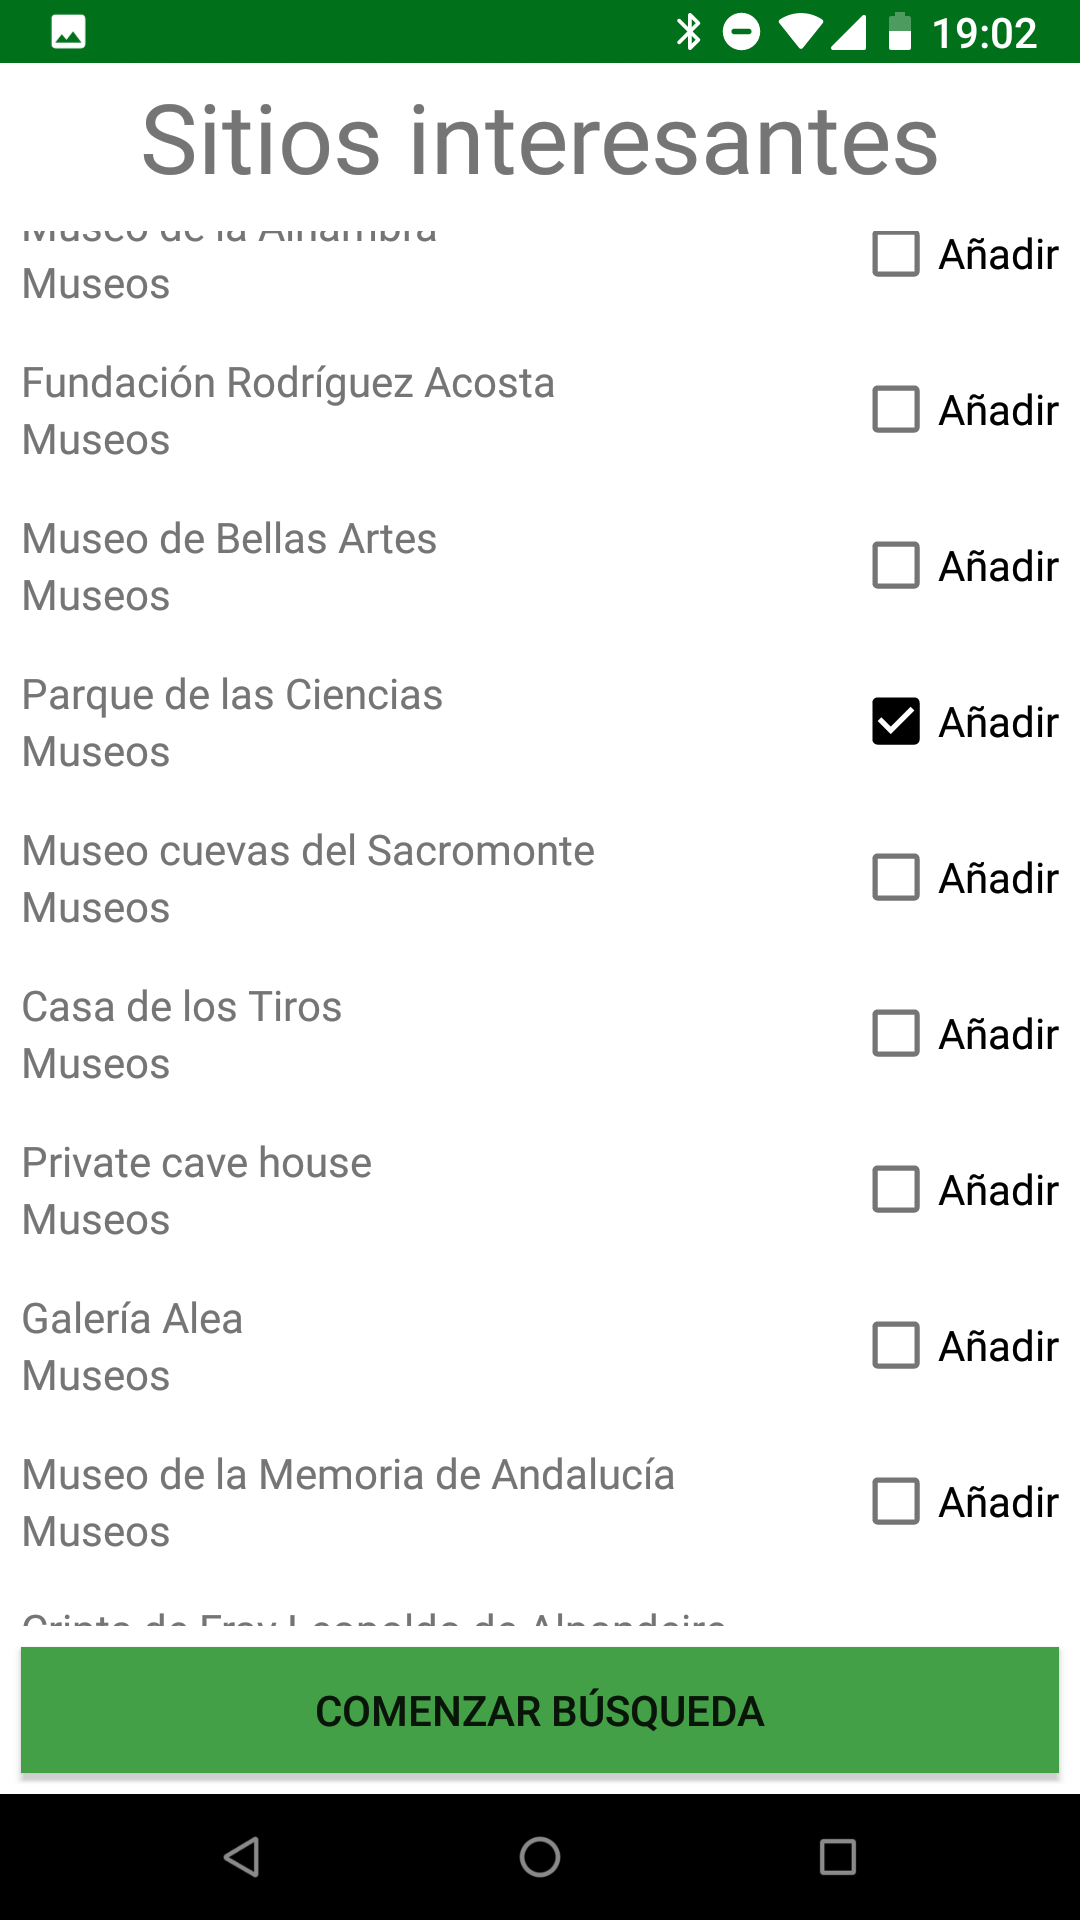
\includegraphics[width=40mm]{imagenes/seleccion_parque}}
	\subfigure{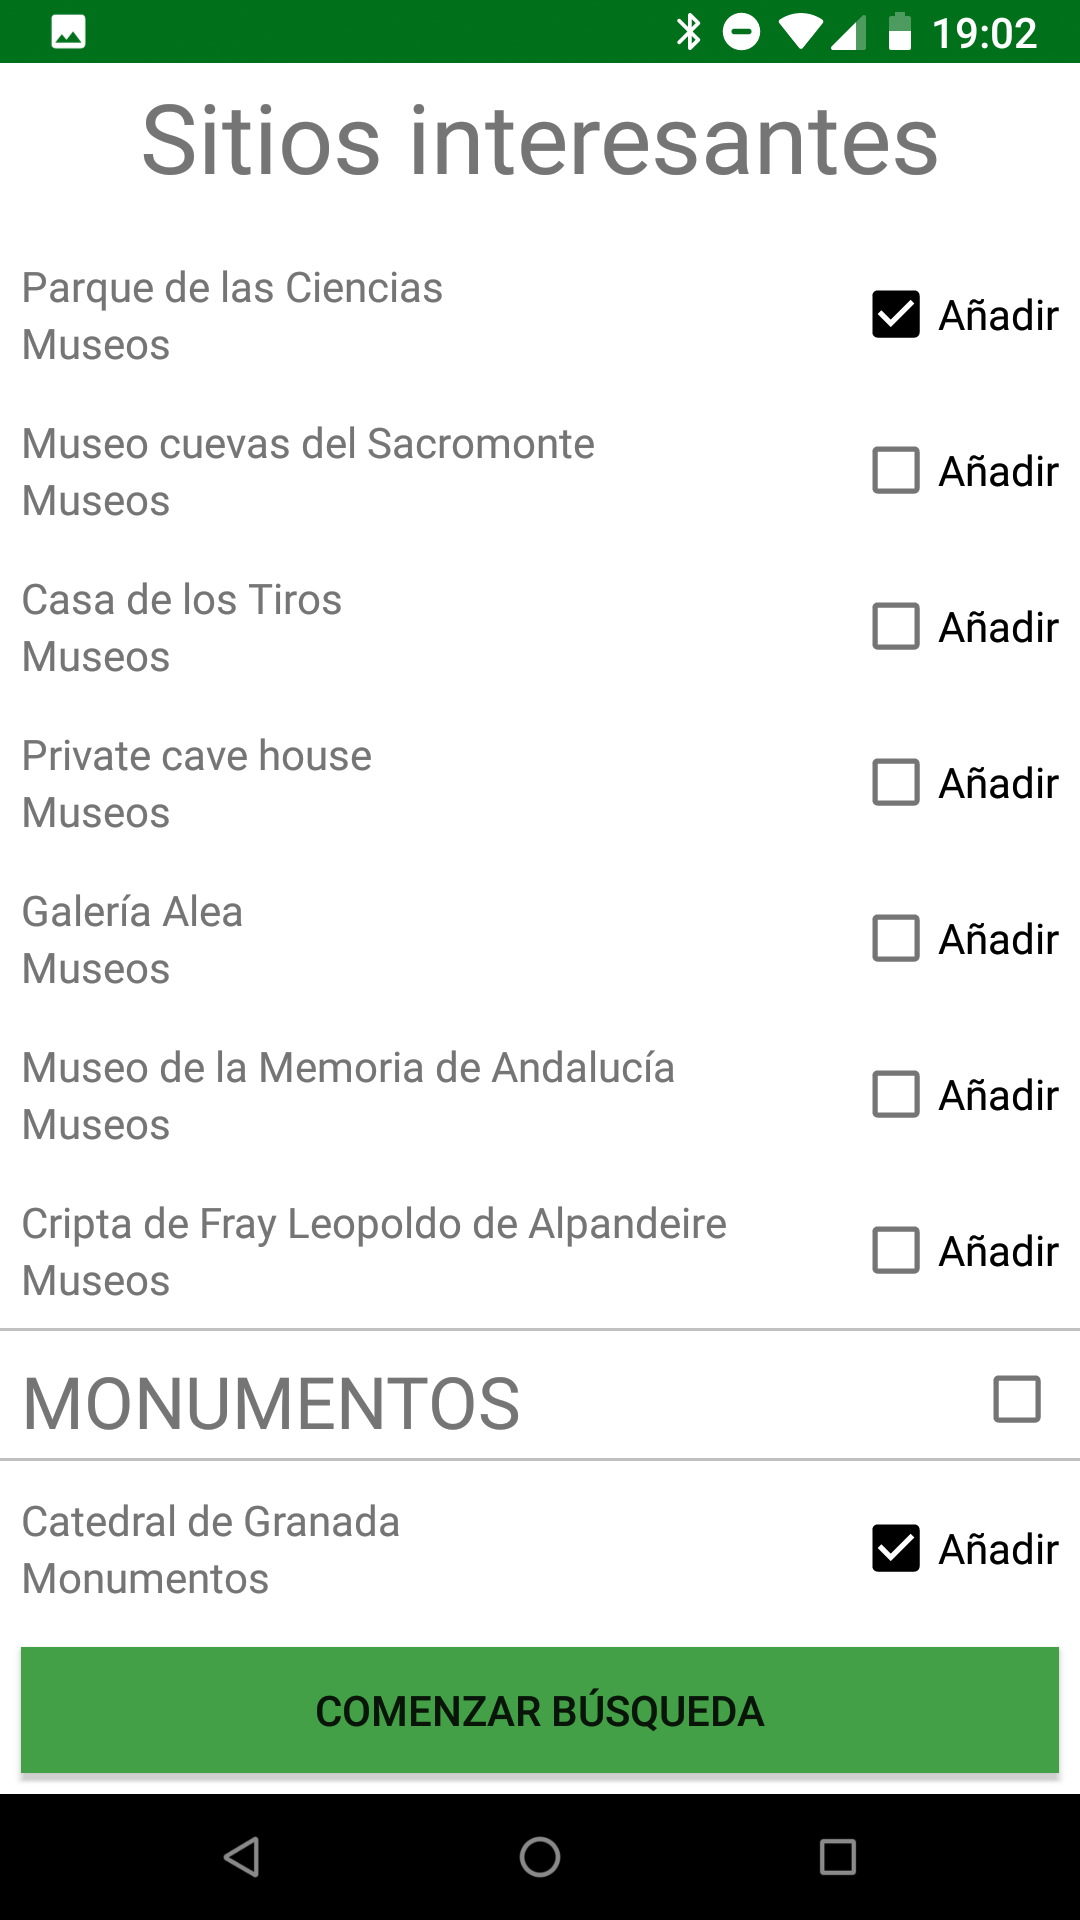
\includegraphics[width=40mm]{imagenes/seleccion_catedral}}
	\caption{Selección de un subconjunto específico de punto de interés.}
	\label{fig:seleccion_multiple}
\end{figure}
\begin{figure}[H]
	\centering
	\subfigure{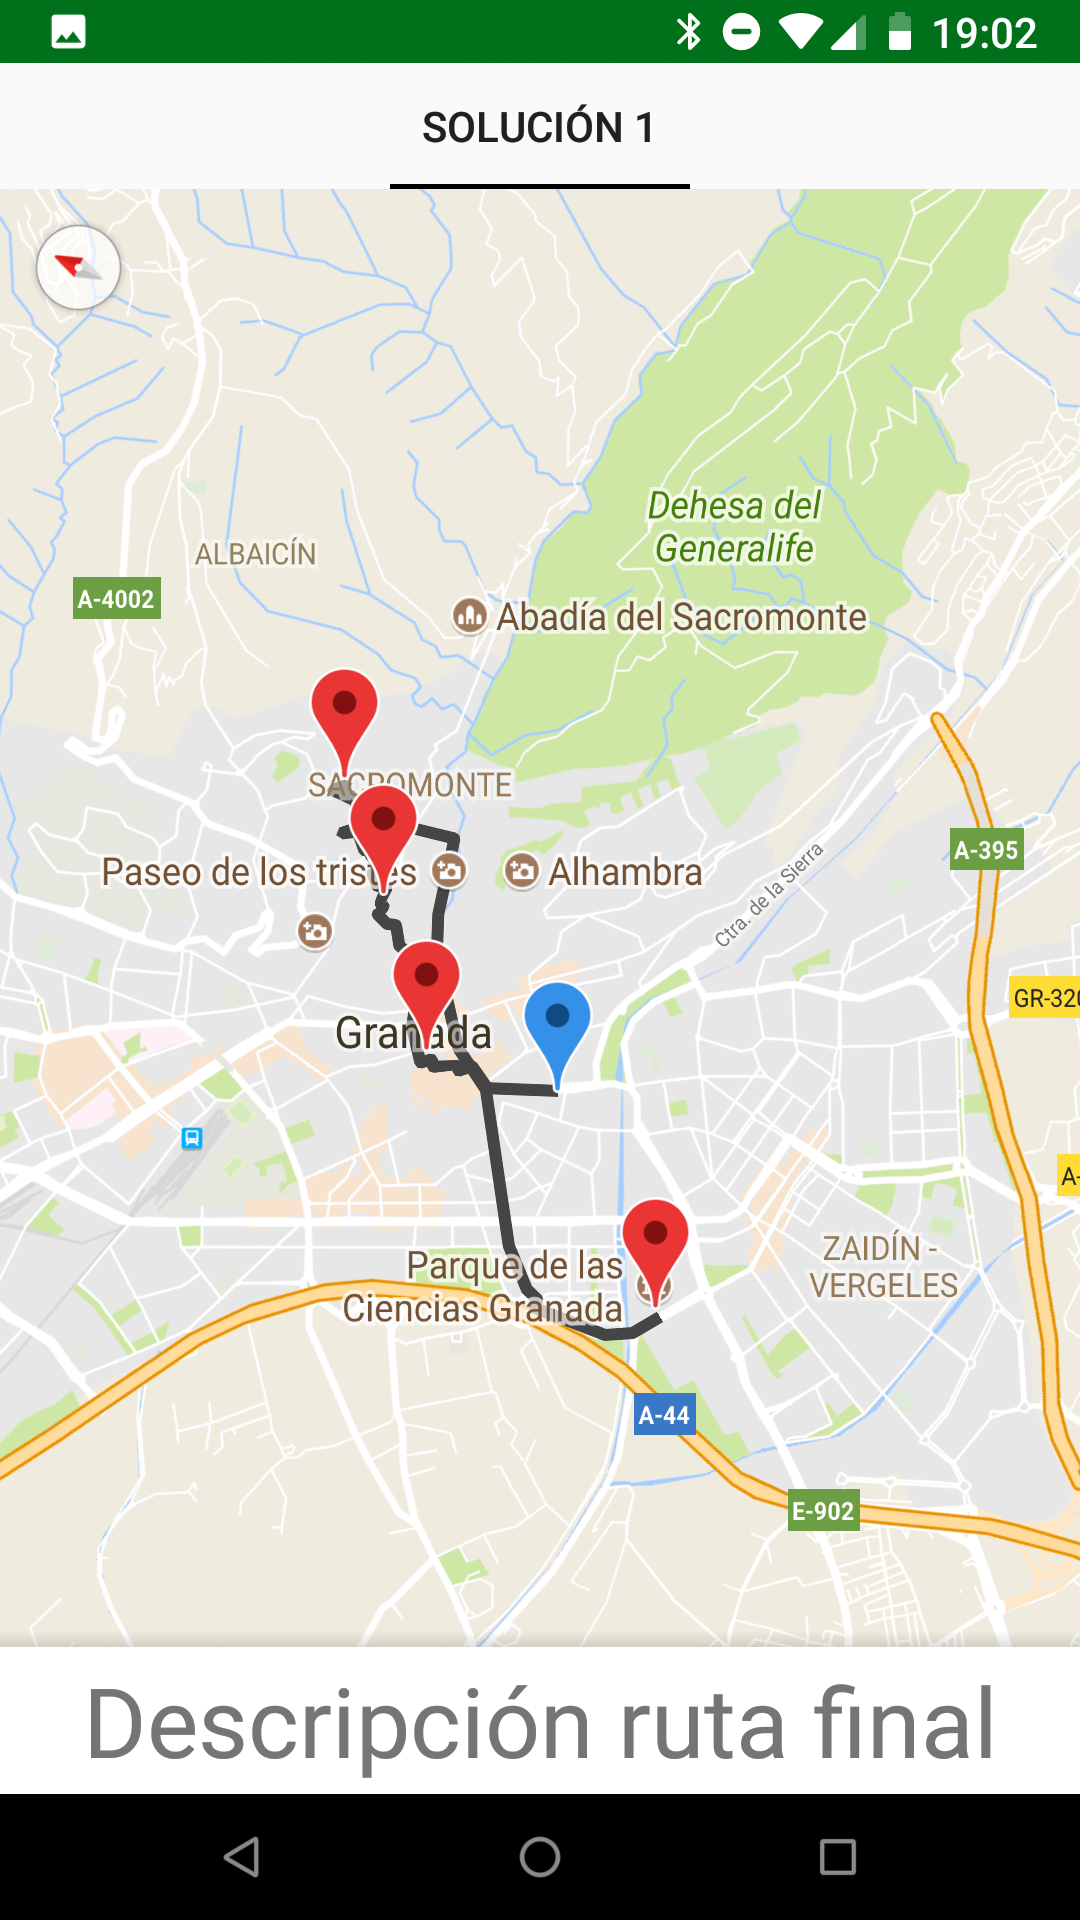
\includegraphics[width=40mm]{imagenes/salida_2}}
	\subfigure{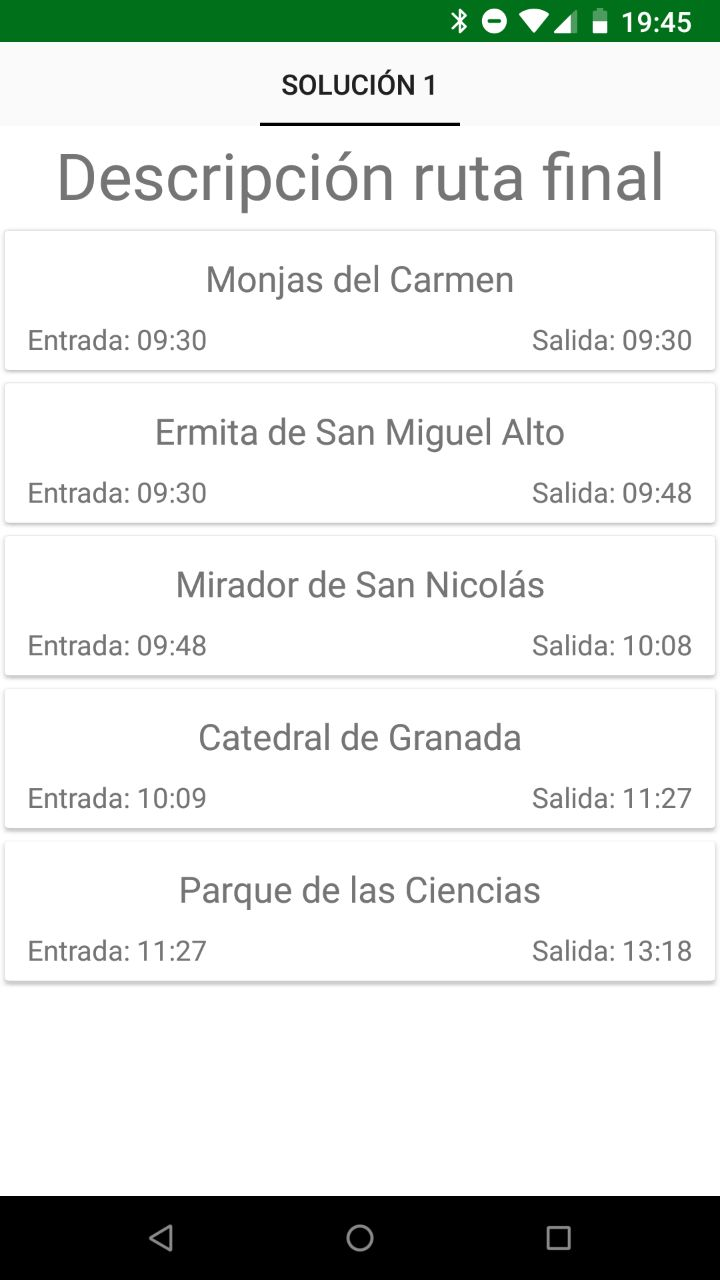
\includegraphics[width=40mm]{imagenes/descripcion_2}}
	\caption{Ruta calculada para el conjunto de puntos de interés.}
	\label{fig:salida_2}
\end{figure}